\documentclass[11pt]{article}

\usepackage{a4wide}
\usepackage{mathptm}
\usepackage{xspace}
\usepackage{amsmath}
\usepackage{graphicx}
\usepackage{algorithm}
\usepackage{algpseudocode}
\usepackage{tikz}
\usepackage{tkz-graph}
\usetikzlibrary{shapes.misc, positioning}
\usepackage{listings}
\usepackage{color}
\usepackage[colorlinks=true,urlcolor=blue]{hyperref}

\definecolor{dkgreen}{rgb}{0,0.6,0}
\definecolor{gray}{rgb}{0.5,0.5,0.5}
\definecolor{mauve}{rgb}{0.58,0,0.82}

\lstset{frame=tb,
  language=Java,
  aboveskip=3mm,
  belowskip=3mm,
  showstringspaces=false,
  columns=flexible,
  basicstyle={\small\ttfamily},
  numbers=left,
  numberstyle=\tiny\color{gray},
  keywordstyle=\color{blue},
  commentstyle=\color{dkgreen},
  stringstyle=\color{mauve},
  breaklines=true,
  breakatwhitespace=true,
  tabsize=3
}
\begin{document}

\title{Project report \\Cloud-IoT Access Control System}

\author{Maksim Ohvrill \& Vladimirs Civilgins}

\maketitle

\renewenvironment{abstract}
 {\small
  \begin{center}
  \bfseries \abstractname\vspace{-.5em}\vspace{0pt}
  \end{center}
  \list{}{%
    \setlength{\leftmargin}{20mm}% <change width
    \setlength{\rightmargin}{\leftmargin}%
  }%
  \item\relax}
 {\endlist}

\begin{abstract}
This report provides full documentation on design \& implementation of
  IoT - cloud access control system. And will briefly explain mindset \& reasoning
  behind access control device implementation on hardware \& software side. As
  well as what technologies \& tools that were used to develop this system. Report
  will conclude on how testing was done and summon up the current status of the project 
  and what experience was achieved.
\newline\newline
Link to the whole project: \url{https://github.com/589664/School_stuff/tree/main/DAT110_workspace/DAT110%20-%20Project%204}
\newline\newline
Implementation of TinkerCAD design (part A) can be found here: \url{https://github.com/589664/School_stuff/tree/main/DAT110_workspace/DAT110%20-%20Project%204/Acess%20control%20device}
\newline\newline
Implementation of REST device client \& service can be found here: 
\newline\url{https://github.com/589664/School_stuff/tree/main/DAT110_workspace/DAT110%20-%20Project%204/dat110-project4-cloudservice/ACCloudService/src/main/java/no/hvl/dat110/ac/restservice}
\newline \& here:
\newline
\url{https://github.com/589664/School_stuff/tree/main/DAT110_workspace/DAT110%20-%20Project%204/dat110-project4-iotdevice/ACIoTDevice/src/no/hvl/dat110/aciotdevice/client}
\newline\newline
Report written in latex can be found here: \url{https://github.com/589664/School_stuff/tree/main/DAT110_workspace/DAT110%20-%20Project%204/project_report/report}


\end{abstract}

%\input{commands}

\newpage 
\section{Introduction}
\label{sec:Introduction}
The system that has been developed in this project consists of two parts. Part A and part B. In part A it has been created the hardware of the system, that represents ACD (access control device). The way it has been implemented, is that it’s running as a simulation of Ardruino board by using TinkerCAD website. That is providing tools for creation of a circuit though a website GUI, and running a simulation based on code provided by the user written in C++ programming language. Concept of ACD is that a motion sensor is getting triggered, the system goes over from locked to waiting mode where we can enter a code by using buttons. If the code is correct the system is set in unlocked mode.   

Part B is implementing a virtual part of ACD that uses HTTP – protocol to connect to a REST (Representational state transfer) based cloud service. Simulation of hardware ACD is later changed to use JavaFX GUI, since TinkerCAD could not provide the connection of circuit design to the internet.

System results in a IoT (internet of things) – cloud solution, that provides connection between ACD and cloud service. This makes it possible to track state change of system by storing locked/unlocked attempts in cloud. Change of access code is also getting tracked.




\section{Access Control Design Model}
\label{sec:ACD_model}

\begin{figure}[h]
  \centering
  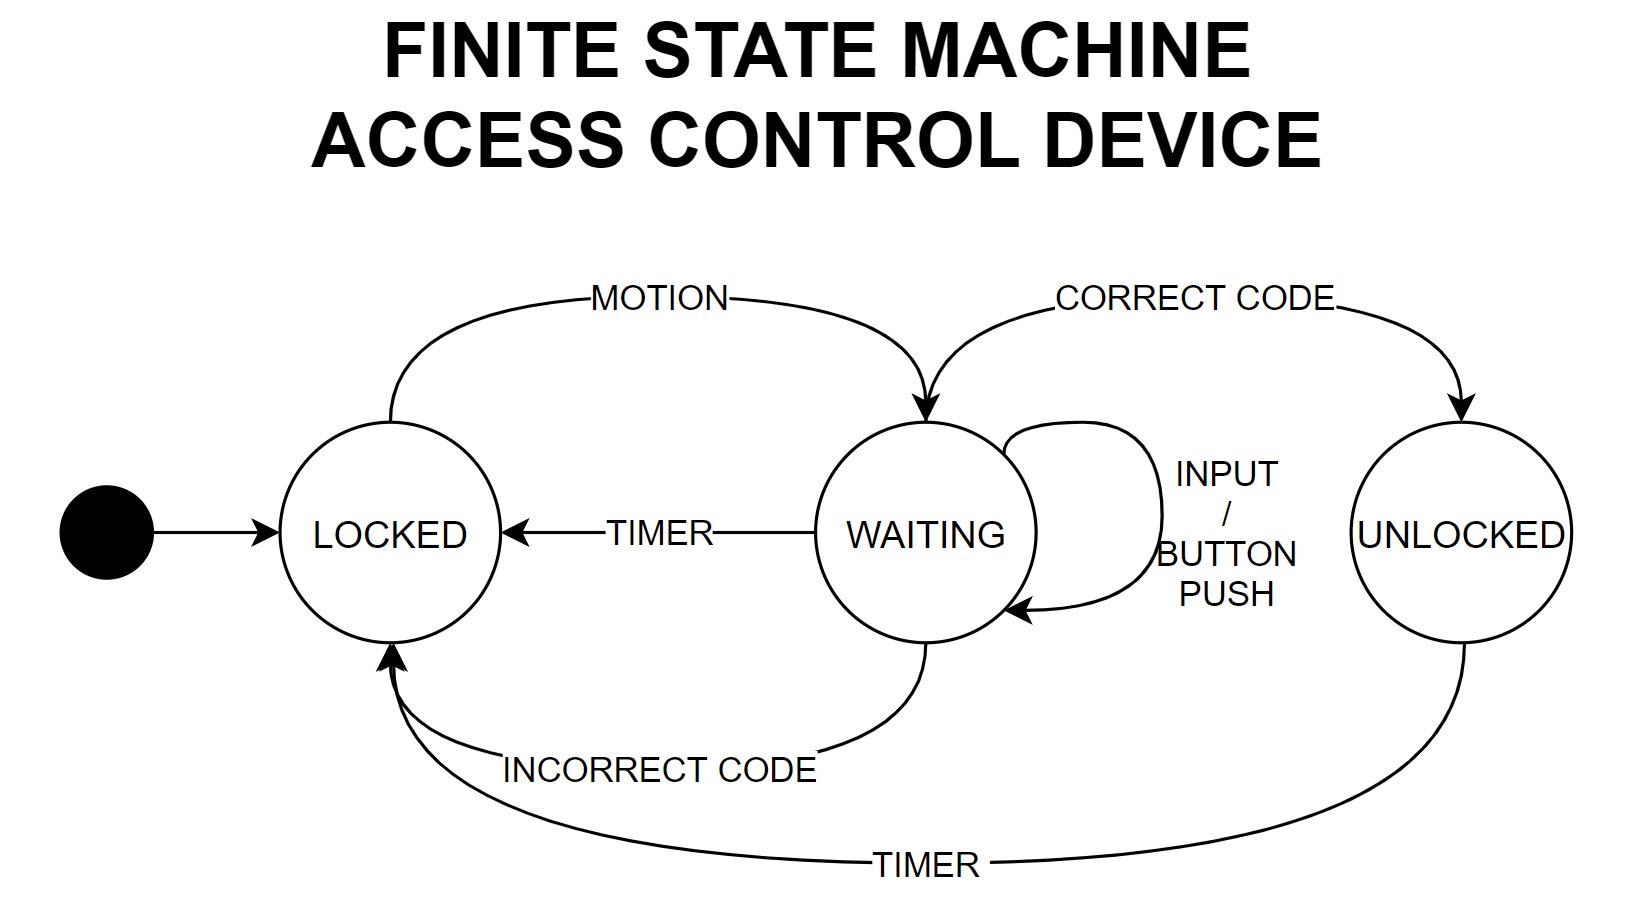
\includegraphics[scale=0.5]{figs/FNS.png}
  \caption{Finite state machine model of access control device}
  \label{fig:framework}
\end{figure}

Design model of ACD was based on the description of functional requirements of the part A. The model contains three states, initial state that is set to locked. Waiting state where input of the access code is taking place. Unlocked state is when entered access code is correct. 
\newline

Motion action is the only thing that can cause the system to go over in waiting state, where access code is entered. That is also the reason behind input loop at waiting state. Further waiting state will go back to locked state if the access code is incorrect, or if the timer ran out and triggered system (optional function). Otherwise, if access code is correct the system is put in unlocked mode, where there’s also a timer that can after an amount of time put the system in locked state.
\newline

Design of the model is drawn as a finite state machine using drawIO UML notation. Where during planning three states, and common main methods of system was taken into account. Input loop at waiting state may seem redundant but describes and helps for the implementation of actual ACD. 




\section{Access Control Hardware/Software Implementation}
\label{sec:ACD_implementation}

Implementation of ACD were performed with use of TinkerCAD that provided GUI for implementation of a circuit that contains an Ardruino board, breadboard, PIR motion sensor, LEDs, pushbuttons, resistors, and wiring. System runs on power of 5V, first thing that was done is connecting two wires for ground and power from Ardruino board to the breadboard. Further PIR – sensor was connected to the system as well, three wires in total two of them for power and grounding. Last one is providing signal and was connected to board at port 11.
\newline\newline

\begin{figure}[h]
  \centering
  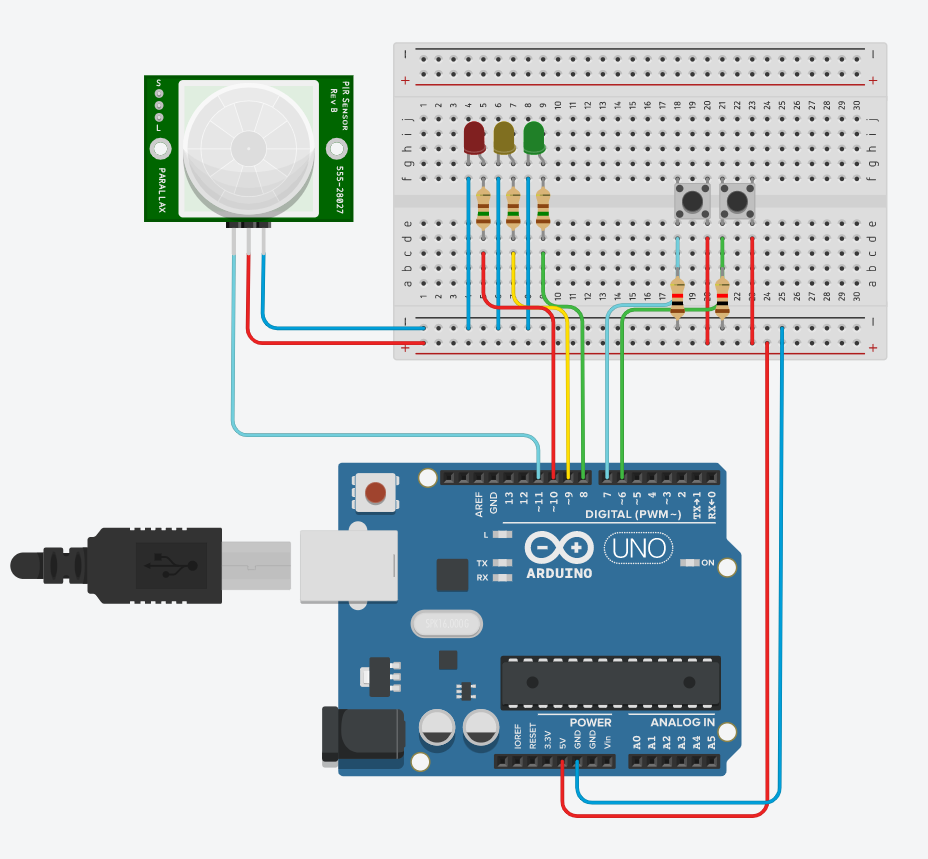
\includegraphics[scale=0.5]{figs/ACD_circut.png}
  \caption{TinkerCAD circuit design of access control device}
  \label{fig:framework}
\end{figure}
For the input of access code, system uses two pushbuttons that has two signal wires connected directly to the Ardruino board, two resistors that is used for grounding. And two wires that is providing power to the push buttons. Last step was to connect the LED bulbs, these are used to display different states of the system. As well as light up when input from the pushbuttons is registered and when the access code from input is incorrect. 
\newline\newline
Red LED bulb is used to indicate incorrect access code setting state of system to locked. As well as locked state that is also initial state. Yellow LED bulb is indicating waiting state of the system, and blink during incoming input on-click from the pushbuttons. Green LED bulb is indicating unlock state for the system. All three LED bulbs are connected with one wire each for grounding, and one wire and resistor each for input signal from the board. Red LED is connected to port 10, yellow led is connected to port 9 and green LED is connected to port 8 at Ardruino board. 

Software implementation of ACD were performed and written using Ardruino version of C++ file format “*.ino” that stand for ending of Ardruino. First part of code is running setup(), where first method that is getting used Serial.begin(9600) method to establish serial communication between Ardruino and another device in this case is our computer. 9600 is the baud rate simply explained this number needs to match on both devices, to be able to send anything over serial. Further we define the pins that is used for input and output on the Ardruino board. 
\newline
After setup() method, we define variables and constants (cannot be modified). For this implementation, the correct access code is hardcoded. States are defined as constants and are not supposed to be changed, the same applies to access code.
\newline\newline
Key part in the code is the method loop() where most of the functionality is taking place. Method is constantly getting called on while simulation is running. States of the system is implemented with use of a switch, where states are represented as cases. The PIR – sensor and the pushbuttons are called with method digitalRead(port number) inside of the loop. Since system needs to constantly monitor if there has been any input on those.  
\newline\newline
There’re three cases that is implemented inside the loop, it is the same ones that is mentioned above locked, waiting and unlock. Logic behind case locked, is that if sensor has been triggered. And there has not been registered a movement before, then system goes over in waiting state. In waiting state there’s several conditions, first one is timer condition. Which sets system in locked state after some time without input. Second and third state is checking for input from pushbuttons and makes the yellow LED blink at push. Input from pushbuttons is padded to string named “current”, that represents input access code. Last two cases checks if the input access code if there’s any, matches the hardcoded valid access code. If the input access code matches hardcoded, system is set in unlocked state. If not, it’s set to locked. 
\newline\newline
For the case unlocked, there’s implemented a timer that after some time in unlocked state. Puts system state back to locked. 


\section{REST API cloud service}
\label{sec:cloud_service}

REST (Representational state transfer)  API (application programming interface) cloud service was implemented with use of “Spark framework”, with documentation provided on this link: 
\newline
\url{http://sparkjava.com/documentation#request}

where it was used simple methods for routes, request, and response. And implementation was based on examples provided in lectures for week 16. The main libraries used for this project are Spark that provides methods mention above. GSON a library that is developed by google and is used to convert java objects into their JSON representation. OkHttp library that provides methods used in rest – client to construct client, request, and response. That is later used to get data from the cloud as for example access code. Or log/post with another words save access entry attempt in cloud. Cloud service is implemented as an Apache maven project, that result in that it can be imported and run without any completion problem on other IDE’s. 
\newline\newline
Documentation for OkHttp is provided here: \url{https://square.github.io/okhttp/}
\newline\newline
Documentation for Gson is provided here: \url{https://sites.google.com/site/gson/gson-user-guide}
\newline\newline
For implementation of routes for ACD, it was used GSON class. Since the data was meant to be returned in JSON representation. 
\newline\newline
Routes implementation:

\begin{itemize}

\item First route “POST /accessdevice/log” it was used toJson() method to convert the result to JSON format, and fromJson() to extract message contained in body from request that was made. Request got the message that was supposed to be added to access – log. And response returned JSON representation of AccessEntry class, that contained both id and the message that was added from request. 

\item Route “GET /accessdevice/log” is meant to get access - log over all entries that has been recorded in cloud. First getting log values that is stored in memory from access – log. And then again simply use GSON class to convert to JSON representation by calling toJson() method.

\item Route “GET /accessdevice/log/:id” is meant to find and get access entry in cloud by the id. The value of parameter id needs to be provided; this was done with help of Postman testing software. First route obtained value of parameter “id” from request, further converting from string to integer. This value is then used on access – log that has a method to find entry by id from ConcurrentHashMap. 

\item Route “GET /accessdevice/code” is meant to get access code from server. AccessCode class is providing get method for that purpose, that is just getting converted to JSON and returned. This route is later used for access device to update access code.

\item Route “PUT /accessdevice/code” is used to update the access code that is stored in cloud service. For this system, access code is limited to input of 2 digits. First, route obtains AccessCode class from body of request that was made and overwrite current access code object in cloud. Then converts it to JSON representation and returns. This route can be used though browser or postman to make a request and change the access code. 

\item Route “DELETE /accessdevice/log” simply deletes all entries that has been saved in cloud by overwriting current access – log object with an empty new one. Empty access – log is returned after being converted to JSON representation. 

\end{itemize}

The access code is stored in cloud, by creating a AccessCode class object. That stores access code in an integer array containing value 1 and 2 at startup. The class also provides a get/set methods and, constructor that is later used to overwrite old AccessCode object. 
\newline

Access – log is implemented in more advanced way, using AtomicInteger that provides mutual exclusive protection. In case of several access attempts is happening at the same time. The entries of access – log is stored using ConcurrentHashMap. That maps “id” integer values to AccessEntry object that also contains identifier integer and message value represented as string. Mapping identifier and entry identifier is same. Identifier in AccessEntry is used for JSON representation, while identifier in HashMap is used as key. Access – log class also provides methods for add, get, clear and JSON representation using GSON class for conversion. 





\section{Device Communication}
\label{sec:device_communication}

Implementation of network communication in ACD is made in RestClient class, as already mentioned with use of OkHttp library that is used to constructs the client, request, and response. This makes it possible for ACD issue requests on the cloud service. For this system there was implemented two methods. First one is doGetAccessCode() that issues HTTP GET request on cloud service to obtain current access code. Method first constructs a client by using OkHttpClient class, this client is later used to make a call and execute a request that results in a response from cloud service. Further method obtains code from response that contains a body. In order to obtain code from the body, method is using fromJson() method from Gson library. Method returns AccessCode object. 
\newline
The way GET request is constructed is with use of OkHttp library that contains Request class, where tha path of the request URL is provided. Together with URL we send path of request to achieve code from cloud service. As mentioned above there’s used "/accessdevice/code" path for that purpose. As well as get() method to specify that it’s a GET request and build() method to build the request. 
\newline\newline
When it comes to POST request, it is also implemented in RestClient class. POST request is some more complex in implementation rather than GET request. And is implemented in method doPostAcessEntry(String message) that suppose to send over the entry as message to cloud service storage (log). Same as previous method it is used client object of OkHttp library to make a call and execute the request. 

POST request is built in the same way as GET request beside that this time it’s used post() method to specify its POST request. This method requires RequestBody that again requires MediaType. MediaType describes the content type of an HTTP request or response body. While RequestBody that converts body of request into java object. For the rest of the implementation, it is the same as GET request method. Both of methods establishes a connection between cloud service and ACD. In that way that ACD can make appropriate HTTP GET and HTTP POST requests. 


\section{System testing}
\label{sec:system_testing}

The IoT cloud system operations were tested with use of API testing tool, mentioned earlier Postman. Hardware part of the IoT system were simulated with use of JavaFX library, that implemented a graphical simulation of the ACD design. 

This allows to make an input though buttons on screen, as well as we can trigger PIR – sensor as a button. At the same time there’s displayed three LED lights that light up accordingly to ACD model design of hardware presented above. This allows interaction on the same level as it would happen in real world. 
\newline\newline
Testing started with starting up cloud service on localhost. Further starting the Postman platform and creating testing request for GET, POST, PUT and DELETE on localhost URL. Then it was just to see if running request returned expected responses. 

After this part was completed then it was time to test if communication between ACD device and cloud service was correctly implemented. In order to do that, cloud service was started up on localhost, further the simulation of ACD device was started up and put into networking mode. That means every entry attempt will be logged in cloud service. 
\newline\newline
Since the system is running as simulation on this machine and are not connected to an any storing internet service. All of entries are saved physically on this machine on the cloud service side. Between every startup all entries from previous session are not getting saved. But the communication is still going though internet using HTTP protocol requests/responses. 

This means system is simulation connection over the internet for testing purposes. After ACD – device is set into networking mode, PIR – sensor is getting triggered and access code is entered. Further if the correct access code was entered, system gets unlocked. Otherwise put back in locked mode. 
\newline\newline
With use of Postman, the access code changing request is getting tested. This request is a PUT request made on localhost, with body containing Json representation of new access code. Last functionality that is tested is if changed access code is stored correctly in the cloud service. Again, running simulation of ACD device put into networking mode, this time entering new access code. There is also a way to check this with a GET request “/accessdevice/code” on cloud service. 

\section{Conclusions}

Concludes on the project, including the technology, its maturity,
learning curve, and quality of the documentation.

The references used throughput the report should constitute a well
chosen set of references, suitable for someone interesting in learning
about the technology.


\bibliographystyle{plain}
\bibliography{report.bib}{}

\end{document}
